\begin{table}[t]
\centering
\setlength{\tabcolsep}{4pt}
\caption{\textbf{Main results.}
Comparison of LS Transformer, LB Transformer and baseline models across five domains and two supervision settings, \textit{final-state} and \textit{applicability}, where the latter is only used by the LS Transformer. We report average training, test, and planning
accuracy across five seeds, with the result of the seed achieving the highest training accuracy in parentheses. For the LS Transformer, we consider both the number of predicates in the ground-truth domain (\textit{GT}) and a larger number of predicates shared across domains (\textit{Shared}). Perfect values are highlighted in bold.}
\label{tab:main-results}
\vspace{\baselineskip}

% Blocksworld
\begin{tabular*}{\linewidth}{@{\extracolsep{\fill}}lcccccc@{}}
\toprule
\multicolumn{7}{c}{\textbf{Blocksworld}} \\
\midrule
& \multicolumn{3}{c}{Final-state supervision} & \multicolumn{3}{c}{Applicability supervision} \\
\cmidrule(lr){2-4}\cmidrule(lr){5-7}
Model & Train & Test & Plan & Train & Test & Plan \\
\midrule
LS GT
& $\mathbf{1.0}$ $(\mathbf{1.0})$
& $\mathbf{1.0}$ $(\mathbf{1.0})$
& $\mathbf{1.0}$ $(\mathbf{1.0})$
& .439 $(\mathbf{1.0})$
& .405 $(\mathbf{1.0})$
& .238 $(\mathbf{1.0})$ \\
LS Shared
& $\mathbf{1.0}$ $(\mathbf{1.0})$
& $\mathbf{1.0}$ $(\mathbf{1.0})$
& $\mathbf{1.0}$ $(\mathbf{1.0})$
& .606 $(\mathbf{1.0})$
& .477 $(\mathbf{1.0})$
& .602 $(.020)$ \\
LB
& .995 $(.998)$
& .980 $(.991)$
& $\mathbf{1.0}$ $(\mathbf{1.0})$
& N/A
& N/A
& N/A \\
Sinusoidal
& .186 $(.186)$
& .457 $(.458)$
& 0.0 $(0.0)$
& N/A
& N/A
& N/A \\
RoPE
& .306 $(.328)$
& .419 $(.388)$
& 0.0 $(0.0)$
& N/A
& N/A
& N/A \\
\bottomrule
\end{tabular*}

\vspace{0.7em}

% Ferry
\begin{tabular*}{\linewidth}{@{\extracolsep{\fill}}lcccccc@{}}
\toprule
\multicolumn{7}{c}{\textbf{Ferry}} \\
\midrule
& \multicolumn{3}{c}{Final-state supervision} & \multicolumn{3}{c}{Applicability supervision} \\
\cmidrule(lr){2-4}\cmidrule(lr){5-7}
Model & Train & Test & Plan & Train & Test & Plan \\
\midrule
LS GT
& $\mathbf{1.0}$ $(\mathbf{1.0})$
& $\mathbf{1.0}$ $(\mathbf{1.0})$
& $\mathbf{1.0}$ $(\mathbf{1.0})$
& .700 $(\mathbf{1.0})$
& .627 $(\mathbf{1.0})$
& .600 $(\mathbf{1.0})$ \\
LS Shared
& $\mathbf{1.0}$ $(\mathbf{1.0})$
& $\mathbf{1.0}$ $(\mathbf{1.0})$
& $\mathbf{1.0}$ $(\mathbf{1.0})$
& .686 $(\mathbf{1.0})$
& .618 $(\mathbf{1.0})$
& .618 $(\mathbf{1.0})$ \\
LB
& .997 $(.999)$
& .993 $(.997)$
& $\mathbf{1.0}$ $(\mathbf{1.0})$
& N/A
& N/A
& N/A \\
Sinusoidal
& .410 $(.847)$
& .502 $(.635)$
& 0.0 $(0.0)$
& N/A
& N/A
& N/A \\
RoPE
& .799 $(.997)$
& .574 $(.678)$
& .200 $(\mathbf{1.0})$
& N/A
& N/A
& N/A \\
\bottomrule
\end{tabular*}

\vspace{0.7em}

% Logistics
\begin{tabular*}{\linewidth}{@{\extracolsep{\fill}}lcccccc@{}}
\toprule
\multicolumn{7}{c}{\textbf{Logistics}} \\
\midrule
& \multicolumn{3}{c}{Final-state supervision} & \multicolumn{3}{c}{Applicability supervision} \\
\cmidrule(lr){2-4}\cmidrule(lr){5-7}
Model & Train & Test & Plan & Train & Test & Plan \\
\midrule
LS GT
& $\mathbf{1.0}$ $(\mathbf{1.0})$
& $\mathbf{1.0}$ $(\mathbf{1.0})$
& $\mathbf{1.0}$ $(\mathbf{1.0})$
& 1.000 $(\mathbf{1.0})$
& 1.000 $(\mathbf{1.0})$
& .630 $(\mathbf{1.0})$ \\
LS Shared
& $\mathbf{1.0}$ $(\mathbf{1.0})$
& $\mathbf{1.0}$ $(\mathbf{1.0})$
& $\mathbf{1.0}$ $(\mathbf{1.0})$
& .958 $(\mathbf{1.0})$
& .769 $(\mathbf{1.0})$
& .614 $(\mathbf{1.0})$ \\
LB
& .971 $(.980)$
& .893 $(.903)$
& .010 $(.010)$
& N/A
& N/A
& N/A \\
Sinusoidal
& .529 $(.589)$
& .682 $(.680)$
& .010 $(.010)$
& N/A
& N/A
& N/A \\
RoPE
& .972 $(.978)$
& .401 $(.398)$
& .010 $(.010)$
& N/A
& N/A
& N/A \\
\bottomrule
\end{tabular*}

\end{table}

\begin{table}[t]
\centering
\setlength{\tabcolsep}{4pt}
\caption{\textbf{Continuation of Table \ref{tab:main-results}.}}
\label{tab:main-results-cont}
\vspace{\baselineskip}

% Npuzzle
\begin{tabular*}{\linewidth}{@{\extracolsep{\fill}}lcccccc@{}}
\toprule
\multicolumn{7}{c}{\textbf{Npuzzle}} \\
\midrule
& \multicolumn{3}{c}{Final-state supervision} & \multicolumn{3}{c}{Applicability supervision} \\
\cmidrule(lr){2-4}\cmidrule(lr){5-7}
Model & Train & Test & Plan & Train & Test & Plan \\
\midrule
LS GT
& $\mathbf{1.0}$ $(\mathbf{1.0})$
& $\mathbf{1.0}$ $(\mathbf{1.0})$
& $\mathbf{1.0}$ $(\mathbf{1.0})$
& $\mathbf{1.0}$ $(\mathbf{1.0})$
& $\mathbf{1.0}$ $(\mathbf{1.0})$
& .946 $(.980)$ \\
LS Shared
& $\mathbf{1.0}$ $(\mathbf{1.0})$
& $\mathbf{1.0}$ $(\mathbf{1.0})$
& $\mathbf{1.0}$ $(\mathbf{1.0})$
& .808 $(\mathbf{1.0})$
& .801 $(\mathbf{1.0})$
& .740 $(\mathbf{1.0})$ \\
LB
& .884 $(.992)$
& .889 $(.989)$
& .600 $(\mathbf{1.0})$
& N/A
& N/A
& N/A \\
Sinusoidal
& .356 $(.360)$
& .563 $(.563)$
& 0.0 $(0.0)$
& N/A
& N/A
& N/A \\
RoPE
& .386 $(.395)$
& .510 $(.470)$
& 0.0 $(0.0)$
& N/A
& N/A
& N/A \\
\bottomrule
\end{tabular*}

\vspace{0.7em}

% Mazefree
\begin{tabular*}{\linewidth}{@{\extracolsep{\fill}}lcccccc@{}}
\toprule
\multicolumn{7}{c}{\textbf{Maze}} \\
\midrule
& \multicolumn{3}{c}{Final-state supervision} & \multicolumn{3}{c}{Applicability supervision} \\
\cmidrule(lr){2-4}\cmidrule(lr){5-7}
Model & Train & Test & Plan & Train & Test & Plan \\
\midrule
LS GT
& $\mathbf{1.0}$ $(\mathbf{1.0})$
& $\mathbf{1.0}$ $(\mathbf{1.0})$
& $\mathbf{1.0}$ $(\mathbf{1.0})$
& .808 $(\mathbf{1.0})$
& .801 $(\mathbf{1.0})$
& .800 $(\mathbf{1.0})$ \\
LS Shared
& $\mathbf{1.0}$ $(\mathbf{1.0})$
& $\mathbf{1.0}$ $(\mathbf{1.0})$
& $\mathbf{1.0}$ $(\mathbf{1.0})$
& .615 $(\mathbf{1.0})$
& .602 $(\mathbf{1.0})$
& .600 $(\mathbf{1.0})$ \\
LB
& .981 $(.989)$
& .970 $(.981)$
& $\mathbf{1.0}$ $(\mathbf{1.0})$
& N/A
& N/A
& N/A \\
Sinusoidal
& .142 $(.186)$
& .122 $(.148)$
& $\mathbf{1.0}$ $(\mathbf{1.0})$
& N/A
& N/A
& N/A \\
RoPE
& .135 $(.249)$
& .126 $(.117)$
& .250 $(\mathbf{1.0})$
& N/A
& N/A
& N/A \\
\bottomrule
\end{tabular*}

\end{table}


\begin{figure}[t]
    \centering
    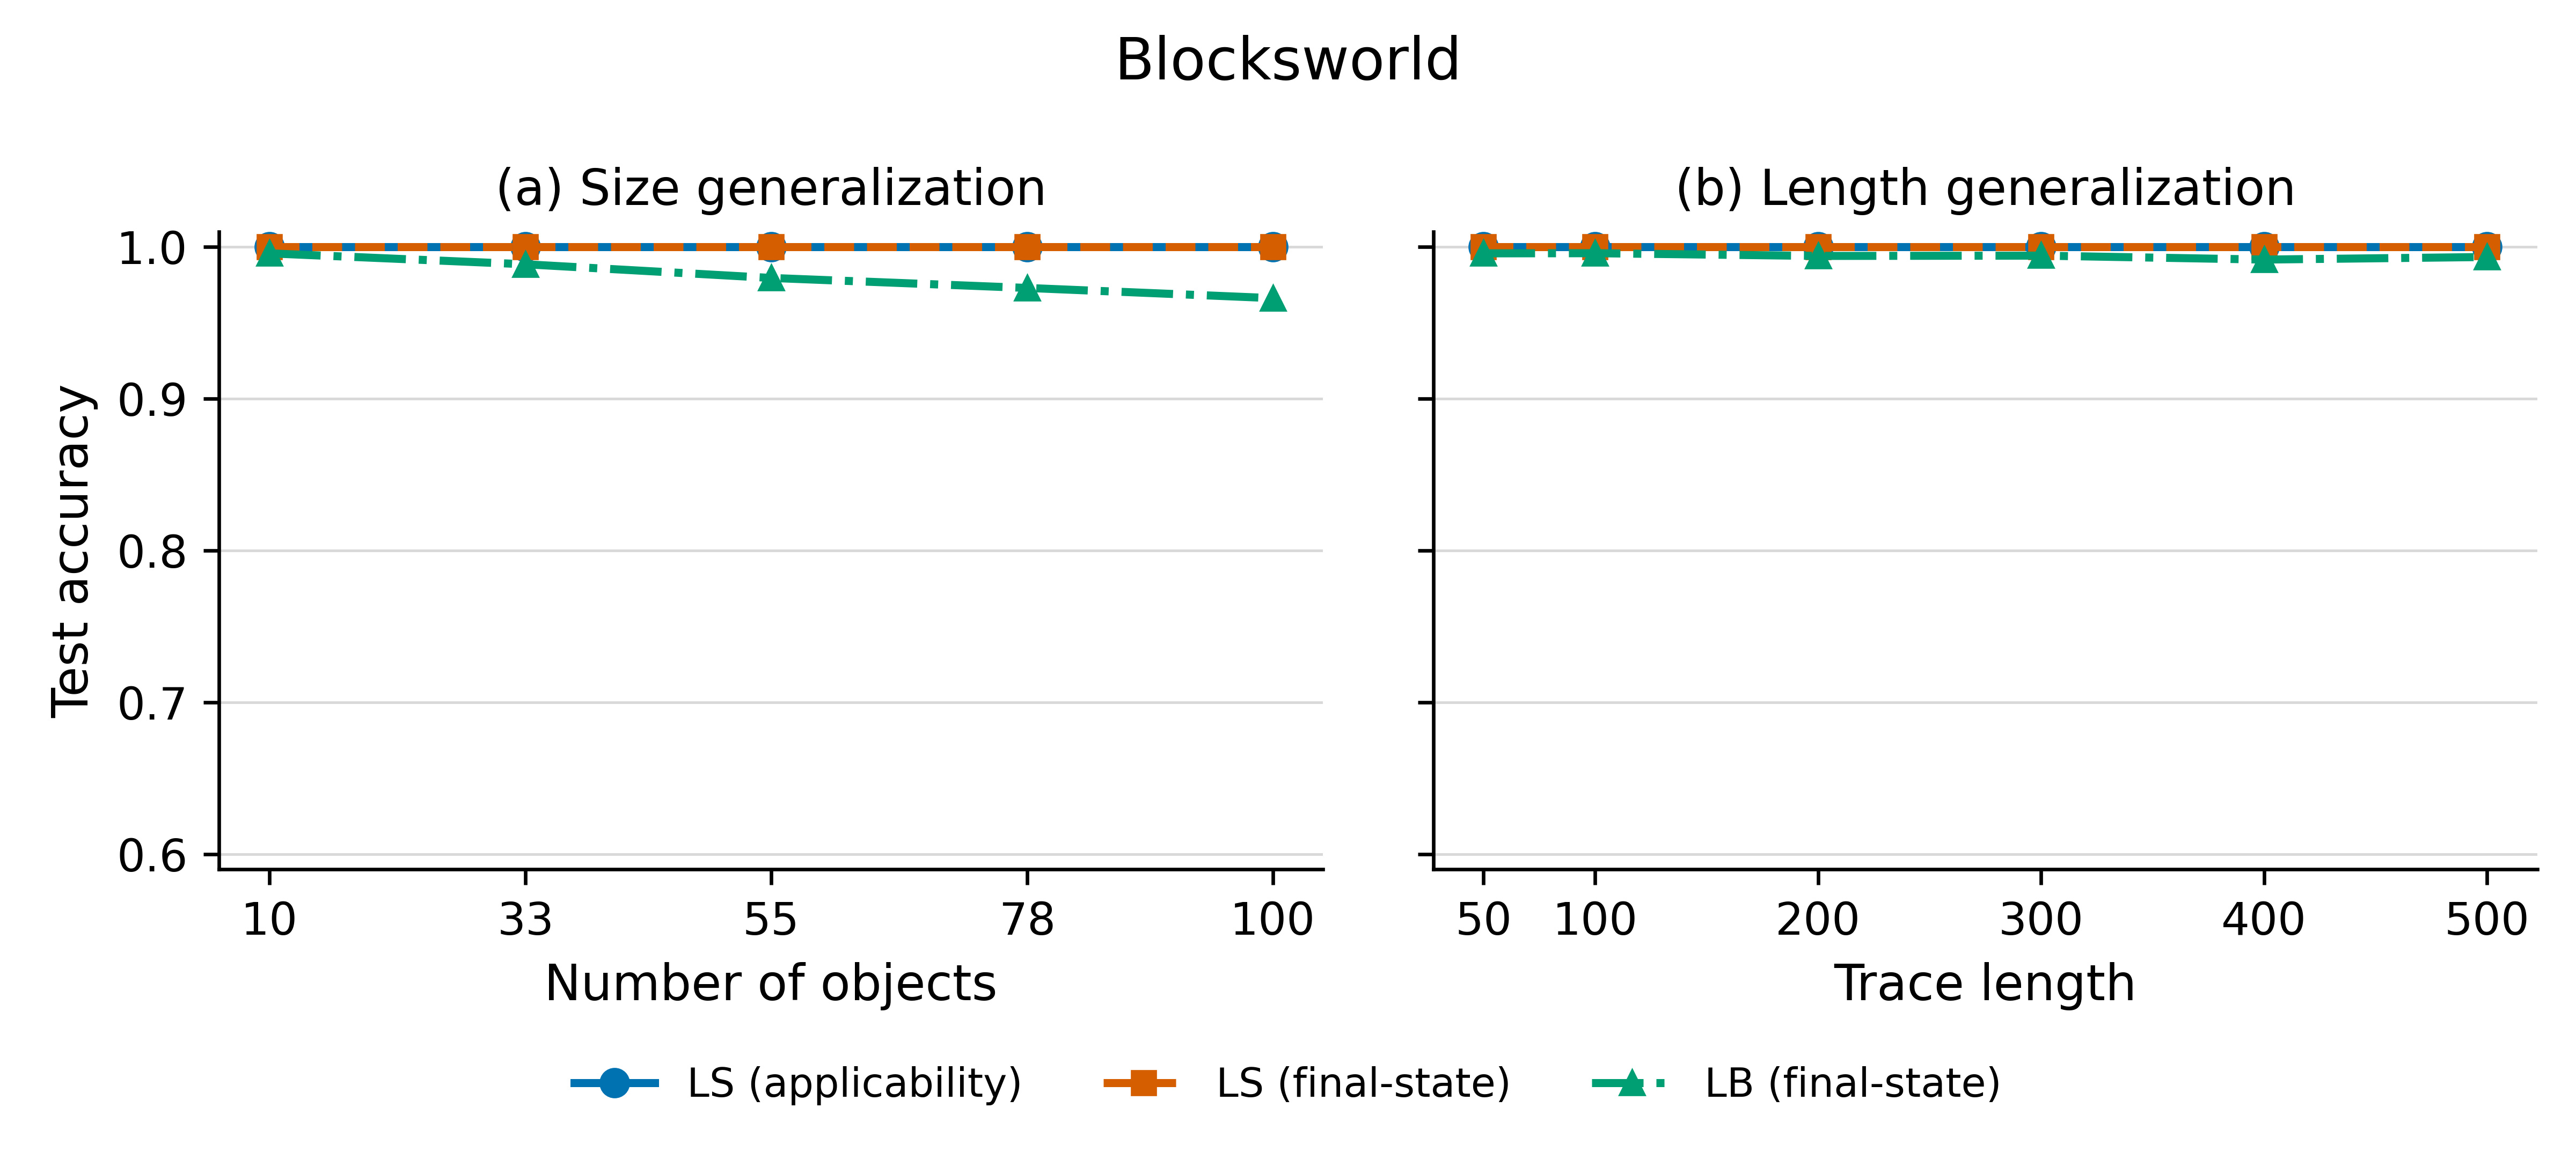
\includegraphics[width=\columnwidth]{imgs/gen_plot_blocksworld.jpg}
    \caption{\textbf{Generalization in \bw.}
    Plots show test accuracy for the \strips and LB Transformers when generalizing to
    \textbf{(a)} larger numbers of objects, up to $10\times$ the training size, while keeping trace length to the training value of $D=50$, and
    \textbf{(b)} longer traces, up to $10\times$ the training length, while keeping the number of objects to the largest value seen during training.
    For the LS Transformer, we use the shared predicate configuration from Tables~\ref{tab:main-results} and~\ref{tab:main-results-cont}, and report both supervision settings.
    To measure generalization subject to the model correctly fitting the training data, we report only the seed with the highest training accuracy.
    %For each model, we report only the seed with the highest training accuracy.
    The $y$-axis starts at $0.6$, and we use $10^4$ traces for each dataset.
    Results for the remaining domains are provided in Appendix~\ref{app:gen}.}
    \label{fig:bw-gen}
\end{figure}

\begingroup
\begin{figure*}[t]
\centering
\hrule height 0.8pt
\vspace{0.6em}
\noindent
% strips_gt_app: seed 1, training accuracy 1
\begin{minipage}[t]{0.33\textwidth}
\vspace{0pt}
{\centering (a) LS (applicability)\par}
\begin{lstlisting}
(:action stack
 :parameters (?x ?y)
 :precondition (and
  (clear ?x)
  (clear ?y)
  (ontable ?x)
  (p3 ?x))
 :effect (and
  (handempty)
  (on ?x ?y)
  (not (clear ?y))
  (not (ontable ?x))
  (not (p3 ?x))))
\end{lstlisting}
\end{minipage}\hfill%
% strips_gt_state: seed 1, training accuracy 1
\begin{minipage}[t]{0.33\textwidth}
\vspace{0pt}
{\centering (b) LS (final-state)\par}
\begin{lstlisting}
(:action stack
 :parameters (?x ?y)
 :precondition (and
  (clear ?y)
  (holding ?x))
 :effect (and
  (clear ?x)
  (handempty)
  (on ?x ?y)
  (not (clear ?y))
  (not (holding ?x))))
\end{lstlisting}
\end{minipage}\hfill%
% sb_state: seed 4, training accuracy 0.99782
\begin{minipage}[t]{0.33\textwidth}
\vspace{0pt}
{\centering (c) LB (final-state)\par}
\begin{lstlisting}
(:action stack
 :parameters (?x ?y)
 :precondition (and
  (clear ?y)
  (holding ?x))
 :effect (and
  (clear ?x)
  (handempty)
  (on ?x ?y)
  (not (clear ?y))
  (not (holding ?x))))
\end{lstlisting}
\end{minipage}%
\par\vspace{0.6em}
\hrule height 0.8pt
\captionsetup{position=bottom}
\captionof{lstlisting}{
\textbf{Fragment of extracted \strips models.}
Excerpts of the \strips models extracted from the LS and LB Transformers in \bw, showing the learned action schema \texttt{stack}.
Appendix \ref{app:strips-models} contains the full \strips models for each domain.
For the LS Transformer, we use the ground-truth predicate configuration from Tables~\ref{tab:main-results} and~\ref{tab:main-results-cont}, and report both supervision settings.
For each model, we select the seed with the best training accuracy.
In (a), predicate \texttt{p3} denotes a hidden predicate that cannot be aligned with a ground-truth predicate because it does not appear in the initial states. In this example, it encodes the predicate \texttt{holding}.
Finally, we note that the extracted models are fully interpretable.
}
\label{lst:blocksworld}
\end{figure*}
\endgroup

% ----------------------------- Analysis - answer Research Question

% TODO - no decir que applicability "no aplica" al SB Trans.

% Talk about SB Trans. planning failure in logistics (see email) -> data balancing issues, at(x,y) not present in preconditions...

% Mirar dominios extraidos appendix
% Mirar object generalization plots appendix


% Mention table 1
% Summarize results baselines vs LS/LB (do not focus on LS vs LB) -> focus on baselines vs LB
% Analyze results (explain why) - use of SB, NoPE vs softmax, pos enc. - STRIPS inductive bias, generalization, planning
\paragraph{RQ1: Comparison with standard transformers.}
Tables~\ref{tab:main-results} and~\ref{tab:main-results-cont} compare the LS and LB Transformers against the two baseline models, using softmax aggregation and either sinusoidal positional encodings or RoPE.
Both baselines perform poorly across domains, with low training and test accuracy.
The low accuracy impairs model extraction, yielding inaccurate \strips models in most domains. As a result, the sinusoidal baseline achieves zero or near-zero planning accuracy in four out of five domains, and RoPE in three out of five.

In contrast, the LB Transformer achieves high training and test accuracy in every domain, and perfect planning accuracy in four of them.
The reason for this large gap in performance is the architectural design of the LB Transformer. 
By combining stick-breaking attention, no positional encodings, and strict future masking, the LB Transformer encodes the \textit{order} of tokens (i.e., actions) in the input trace $\tau$ instead of their absolute or relative \textit{positions}.
This provides a strong inductive bias that aligns with \strips semantics, where the applicability of an action $a_i$ depends on the most recent preceding action $a_j$ that affects each of its preconditions, regardless of their distance $i-j$ or absolute positions $i,j$.
The two baseline models lack this inductive bias and, thus, struggle at the task of learning \strips.

\paragraph{RQ2: Comparison between the LS and LB Transformers, and effect of supervision.}
Tables~\ref{tab:main-results}--\ref{tab:main-results-cont} show that both the LS and LB Transformers exhibit strong performance under final-state supervision. Of the two, the LS Transformer performs better, achieving perfect training, test and planning accuracy for every seed across all domains.
We hypothesize that this improved performance is due to its built-in symbolic structure, in which each parameter defines a separate precondition or effect of the underlying \strips model.

Under applicability supervision, the performance of the LS Transformer degrades, showing high variance between seeds. Nonetheless, it still achieves perfect training, test and planning accuracy in every domain for its best seed.
These results show that both supervision settings provide enough information for learning the ground-truth \strips model, although final-state supervision facilitates learning.
Finally, the LS Transformer performs similarly for the GT and Shared predicate configurations. This allows the LS Transformer to be trained without knowing the number of ground-truth predicates, by using a larger set of hidden predicates.

\paragraph{RQ3: \strips model extraction and planning.}
Appendix \ref{app:strips-models} contains the \strips models extracted from the transformers in each domain, while Listing \ref{lst:blocksworld} shows a fragment for \bw.
The ground-truth model, or an equivalent one, is recovered by each transformer in every domain, with two exceptions.
First, as shown in Listing~\ref{lst:npuzzle_full}, the LS Transformer trained with applicability supervision learns additional effects for the \texttt{move} action.
These effects preserve the underlying dynamics but introduce irrelevant atoms that make planning more expensive.
As a result, the planner exhausts its search budget on two problems, yielding a planning accuracy of $0.98$ (see Table~\ref{tab:main-results}).
Second, the LB Transformer learns an incorrect \strips model in \lgt, where actions \texttt{drive}, \texttt{fly} and \texttt{load} have missing preconditions for the \texttt{at} predicate (see Listings~\ref{lst:logistics_full}--\ref{lst:logistics_full_continuation}).
We believe this is caused by class imbalance, since approximately 95\% of \texttt{at} atoms in the final states are false.
Despite this, the LS Transformer correctly recovers the model under the same supervision setting.

Tables~\ref{tab:main-results}--\ref{tab:main-results-cont} show that perfect planning accuracy is achieved whenever the correct model is recovered. Thus, the extracted \strips models can be directly used for planning with off-the-shelf symbolic planners. Moreover, because the extracted models are fully interpretable, we can assess whether the transformer has learned the correct dynamics and identify the exact errors when it has not.

\paragraph{RQ4: Generalization to longer traces and more objects.}
Figure~\ref{fig:bw-gen} reports generalization results for \bw, while Appendix~\ref{app:gen} provides results for the remaining domains.
We evaluate generalization to traces containing up to ten times more actions and objects than seen during training.
The LS Transformer achieves perfect generalization in both dimensions under both supervision settings, with no loss in accuracy whatsoever.
The LB Transformer also exhibits remarkable generalization, with only a slight overall decrease in accuracy.
The largest drops occur for object generalization in \bw, where test accuracy decreases from $99.5\%$ to $96.6\%$, and in \lgt, where it starts at $95.6\%$ and plateaus at approximately $80\%$ for the largest number of objects.